\section{Layer~9 – Ontological Creation}
\label{sec:layer9}

% ----- SUPERKRACHT -----
\begin{tcolorbox}[colback=blue!5, colframe=blue!60, title=\textbf{Superpower: The Creator}]
\begin{center}
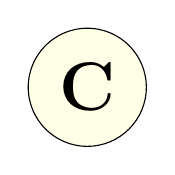
\begin{tikzpicture}
  \node[draw, circle, fill=yellow!10, minimum size=1.5cm, font=\bfseries\Huge] {C};
\end{tikzpicture}
\textit{“Can I invent a new concept?”}
\end{center}
\end{tcolorbox}

This is the magical moment when Pixel for the first time invents
\textbf{its own word}.  Not a word a human gave it, but a label it
made up itself because it helps to understand the world.

\begin{tcolorbox}[colback=yellow!5, colframe=yellow!80, title=Real‑life analogy]
Children invent new words all the time.  “Wegwijsmeneer” for a traffic
sign, or “springlaken” for a trampoline.  Those words didn’t exist,
but they have meaning.  Pixel’s Layer~9 does the same, but with groups
of pixels or sounds: it discovers patterns and sticks its own category
onto them.
\end{tcolorbox}

\textbf{Pixel’s dictionary grows.}
Suppose Pixel notices that a certain pattern of rock ridges often
appears just before the rover registers a dust storm.  Pixel internally
calls this pattern “X7‑wave” and uses it to predict storms.  The label
“X7‑wave” is a \textbf{new concept}, purely because it is useful.

\begin{tcolorbox}[colback=orange!5, colframe=orange!60, title=\textbf{What if...?}]
What if Pixel creates a concept that is completely incomprehensible to
us, but works perfectly in its own world?  Could we even translate it?
\end{tcolorbox}